%- HandOut Flag -----------------------------------------------------------------------------------------
\newif\ifHandout

%- D0cum3nt ----------------------------------------------------------------------------------------------
\documentclass[beamer,10pt]{standalone}   
%\documentclass[beamer,10pt,handout]{standalone}  \Handouttrue  

%- HandOut Flag -----------------------------------------------------------------------------------------
\ifHandout
	\setbeameroption{show notes} %print notes   
\fi

	
%- Packages ----------------------------------------------------------------------------------------------
\usepackage{custom-style}
\usetikzlibrary{positioning}
\usepackage{multicol}


%--Beamer Style-----------------------------------------------------------------------------------------------
\usetheme{toninus}
\usepackage{animate}
\usetikzlibrary{positioning, arrows}
\usetikzlibrary{shapes}
\usetikzlibrary{calc}
\usetikzlibrary{backgrounds}
  \tikzset{
    invisible/.style={opacity=0},
    visible on/.style={alt=#1{}{invisible}},
    alt/.code args={<#1>#2#3}{%
      \alt<#1>{\pgfkeysalso{#2}}{\pgfkeysalso{#3}} % \pgfkeysalso doesn't change the path
    },
  }
 \usetikzlibrary{shapes.misc} 

  
  
\begin{document}

%-------------------------------------------------------------------------------------------------------------------------------------------------
\begin{frame}[t]{Symmetries: intuition}
	\begin{itemize}
		\item (elementary) symmetry: property of a geometric figure (shape) to be invariant under certain transformations.
	\end{itemize}
	\vfill
	\begin{center}
		\resizebox{\textwidth}{!}{			
			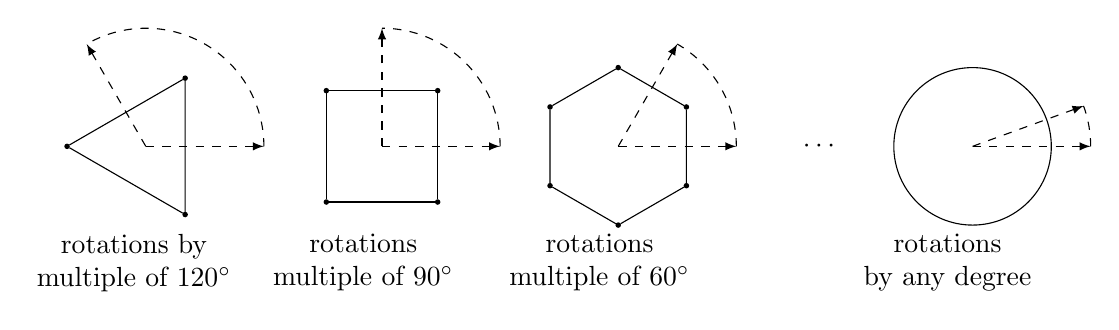
\begin{tikzpicture}
				\pgfmathtruncatemacro\R{1};
				\pgfmathsetmacro\Rext{1.5};
				\pgfmathsetmacro\dist{2*\Rext};
			    \draw[draw=none] (-\Rext,-1) rectangle (\Rext,\Rext);
		
				% Triangle
				\coordinate (o1) at (0,0);
				\draw[draw=none] (o1) -- (60:\R) node[circle, fill, minimum size=2pt,inner sep=0pt, outer sep=0pt](t1){};
				\draw[draw=none] (o1) -- (180:\R) node[circle, fill, minimum size=2pt,inner sep=0pt, outer sep=0pt](t2){};
				\draw[draw=none] (o1) -- (-60:\R) node[circle, fill, minimum size=2pt,inner sep=0pt, outer sep=0pt](t3){};
					
				\draw[dashed,-latex] (o1) -- (0:\Rext);
				\draw[dashed,-latex] (o1) -- (120:\Rext);
				\draw[dashed] (0:\Rext) arc(0:120:\Rext);
								
				\draw (t1) -- (t2) -- (t3) -- (t1);
				
				\node[below right,align=center,thick,outer sep=0pt,visible on=<2->] at (-\Rext,-1)
       				{rotations by\\ multiple of $120^\circ$};


				% Square	
				\coordinate (o2) at (\dist,0);
				\draw[draw=none] (o2) -- ++ (45:\R) node[circle, fill, minimum size=2pt,inner sep=0pt, outer sep=0pt](s1){};
				\draw[draw=none] (o2) -- ++ (135:\R) node[circle, fill, minimum size=2pt,inner sep=0pt, outer sep=0pt](s2){};
				\draw[draw=none] (o2) -- ++ (225:\R) node[circle, fill, minimum size=2pt,inner sep=0pt, outer sep=0pt](s3){};
				\draw[draw=none] (o2) -- ++ (315:\R) node[circle, fill, minimum size=2pt,inner sep=0pt, outer sep=0pt](s4){};
		
					
				\draw[dashed,-latex] (o2) -- ++ (0:\Rext);
				\draw[dashed,-latex] (o2) -- ++ (90:\Rext);
				\draw[dashed] (o2)++(0:\Rext) arc (0:90:\Rext);
								
				\draw (s1) -- (s2) -- (s3) -- (s4) -- (s1);	

				\node[below right,align=center,thick,outer sep=0pt,visible on=<2->] at (-\Rext+\dist,-1)
       				{rotations \\ multiple of $90^\circ$};

				%pentagon
				\coordinate (o3) at (2*\dist,0);
				\draw[draw=none] (o3) -- ++ (30:\R) node[circle, fill, minimum size=2pt,inner sep=0pt, outer sep=0pt](h1){};
				\draw[draw=none] (o3) -- ++ (90:\R) node[circle, fill, minimum size=2pt,inner sep=0pt, outer sep=0pt](h2){};
				\draw[draw=none] (o3) -- ++ (150:\R) node[circle, fill, minimum size=2pt,inner sep=0pt, outer sep=0pt](h3){};
				\draw[draw=none] (o3) -- ++ (210:\R) node[circle, fill, minimum size=2pt,inner sep=0pt, outer sep=0pt](h4){};
				\draw[draw=none] (o3) -- ++ (270:\R) node[circle, fill, minimum size=2pt,inner sep=0pt, outer sep=0pt](h5){};
				\draw[draw=none] (o3) -- ++ (330:\R) node[circle, fill, minimum size=2pt,inner sep=0pt, outer sep=0pt](h6){};
		
		
				\draw[dashed,-latex] (o3) -- ++ (0:\Rext);
				\draw[dashed,-latex] (o3) -- ++ (60:\Rext);
				\draw[dashed] (o3)++(0:\Rext) arc (0:60:\Rext);
								
				\draw (h1) -- (h2) -- (h3) -- (h4)-- (h5) -- (h6) -- (h1);				
				
				\node[below right,align=center,thick,outer sep=0pt,visible on=<2->] at (-\Rext+2*\dist,-1)
       				{rotations \\ multiple of $60^\circ$};
       				
       			\node[] at (2.85*\dist,0) {$\cdots$};				

				\coordinate (o4) at (3.5*\dist,0);			
				\draw[,visible on=<3->] (o4) circle (1);
				\draw[dashed,-latex,visible on=<3->] (o4) -- ++ (0:\Rext);
				\draw[dashed,-latex,visible on=<3->] (o4) -- ++ (20:\Rext);
				\draw[dashed,visible on=<3->] (o4)++(0:\Rext) arc(0:20:\Rext);
				\node[below right,align=center,thick,outer sep=0pt,visible on=<3->] at (-\Rext+3.5*\dist,-1)
       				{rotations \\ by any degree};				
			
			\end{tikzpicture}	
		}
	\end{center}
	\vfill
	\begin{itemize}
		\item<2-> 	Intuitive notion of symmetry is discrete.
		\item<3-> 	Mechanical systems possess "continuous" symmetries.
					\vfill
					\alert{ Keyword: Lie Groups.}
	\end{itemize}
	
\end{frame}
\note[itemize]{
	\item in contrast to the intutive notion of symmeties that might come to one's mind (discrete) - like the mirror symmetry of a butterflies or the radial symmetry of flowers- mechanical systems have continuous symmetries.
	\item e.g. pendulum has rotation symmetries.
}
%-------------------------------------------------------------------------------------------------------------------------------------------------

%-------------------------------------------------------------------------------------------------------------------------------------------------
\begin{frame}[t]{Symmetries: Geometric mechanics}
	\begin{itemize}
		\item Consider a phase space $M$ (symplectic manifold) e.g. a Torus.
	\end{itemize}
	%
	\vfill
	\begin{columns}
    	\begin{column}{.5\textwidth}
			\center
			\includegraphics<1>[width=.75\textwidth]{Pictures/torus2}
			\includegraphics<2>[width=.75\textwidth]{Pictures/arnoldcat-frame/arnoldclown-0.png}
				\only<3->{	
					\animategraphics[autoplay,palindrome,width=.75\textwidth]{2}{Pictures/arnoldcat-frame/arnoldclown-}{0}{3}
				}
		\end{column}
    	\begin{column}{.5\textwidth}
    		\only<2>{
	    		\emph{For the sake of representation,\\
	    		label each state with a color.
	    		\\
	    		e.g. glue a picture on the surface}
	    		\center
				\includegraphics[width=.5\textwidth]{Pictures/clown.png}
			}
			\only<3->{
				Arnold's cat map
				\\
				\tiny
				\url{https://faculty.math.illinois.edu/~palmore/math351-n1/catmap.htm} 
			}
		\end{column}
	\end{columns}
	\vfill
	\onslide<3->{
	\begin{defblock}[Transformation]
		Smooth family of mappings from $M$ into itself.\\
		(Lie group smoothly acting on $M$)
	\end{defblock}
	}
	\vfill
	\onslide<4->{
	\begin{defblock}[Symmetry]
		Is a transformation preserving the symplectic structure of $M$.
	\end{defblock}	
	}

\end{frame}
\note[itemize]{
	\item considero una varietà simplettica,per esempio il toro (è orientabile e 2d quindi ogni forma volume è una forma simplettica)
	\item Observe: A trasformation acts (transform) observables (via pullback) and hamiltonian vector field (via push forward)
	\item loosely speaking a symmetry is a trasformation such that:
		given an observable $o$ with Ham. vec. field $x$, the ham. vec field $\bar{x}$ of the transformed observable $o'$ coincides with the transformation $x'$ of $x$.
	\item questo è un po' improrio, di solito si definisco trasformazioni canoniche le trasformazioni che preservano la struttura simplettica e simmetrie le trasformazioni canoniche che preservano anche la fissata hamiltoniana.
	\item formally symmetries are described by Lie group actions on configuration spaces or phase spaces.
	\item their importance lies in the associated conserved quantites and the reduced description that arise from them.

		
}
%-------------------------------------------------------------------------------------------------------------------------------------------------

%-------------------------------------------------------------------------------------------------------------------------------------------------
\begin{frame}[t]{Hamiltonian Symmetries: comomentum maps}
	\begin{block}{Recall: gist of the symplectic structure}
			
\begin{tikzpicture}[
				node distance=0.35\linewidth,
				]
				\node [text width=0.15\linewidth,rectangle] (lhs) {for any \\ observable};
				\node [text width=0.2\linewidth, rectangle,right of=lhs] (chs) {associated \\ Ham. Vec. field};
				\node [text width=0.4\linewidth, rectangle,right of=chs,node distance=.45\linewidth] (rhs) {associated transformation\\ (integrating the flow)};
				\draw[-stealth,decorate,decoration={snake}] (lhs) -- (chs);
				\draw[-stealth,decorate,decoration={snake}] (chs) -- (rhs);
			\end{tikzpicture}
	\end{block}
	%
	\vfill
	\onslide<2->{
		\begin{defblock}[Hamiltonian symmetry]
			Transformation obtainable as a flow of a certain observable quantity ("generalized momentum").
			\\
			Mathematically, existence of a certain function called \emph{comomentum map}.
		\end{defblock}
	}
	\vspace{-.5em}
	\begin{columns}
    	\begin{column}[t]{.5\textwidth}
			\only<3->{
			\begin{exblock}[Angular momentum $L$]
					\center
					\resizebox{.9\textwidth}{!}{
						\pgfmathtruncatemacro\steps{8}
						\pgfmathtruncatemacro\mintheta{-170}
						\pgfmathtruncatemacro\maxtheta{-90}
						\pgfmathsetmacro\deltatheta{(\maxtheta-\mintheta)/(\steps-1)}
						\pgfmathsetmacro\viewpitch{30}
						\pgfmathsetmacro\diam{2}
						\pgfmathsetmacro\H{4}
						\pgfmathsetmacro\deltaH{.5}
						\pgfmathsetmacro\X{\diam}
						\pgfmathsetmacro\Y{\diam*sin(\viewpitch)}	
						\pgfmathsetmacro\vel{\diam/4}	
						\begin{animateinline}[autoplay,loop]{6} % 5 fps, same as 0.2 s transduration
							\multiframe{\steps}{i=0+1}{
								\begin{tikzpicture}
									\pgfmathsetmacro\theta{\mintheta + \i*\deltatheta}
									\draw[green,dashed,fill=green!20] (0,0) ellipse ({\X} and {\Y});
									%\draw [blue,dashed] (-1.25,-3.5) arc (180:360:1.25 and -0.5);
									\draw[green,dashed,fill=green!20] (0,-{\H}) ellipse ({\X} and {\Y});
									\draw [blue,dashed] (-{\X},-{.5*\H}) arc (180:360:{\X} and -{\Y});
									\draw [green](-{\X},0) -- (-{\X},-{\H});
									\draw [green]({\X},-{\H}) -- ({\X},0);  
									\fill [green!80,opacity=0.5] (-{\X},0) -- (-{\X},-{\H}) arc (180:360:{\X} and {\Y}) -- ({\X},0) arc (0:180:{\X} and -{\Y});
									\draw [blue](-\X,-{.5*\H}) arc (180:360:{\X} and {\Y});
									\foreach \h in {0,-\deltaH,...,-\H}{
										\draw[red,-stealth] (0,\h)++({cos(\theta)*\X},{sin(\theta)*\Y}) --++({-\vel*sin(\theta)},{\vel*cos(\theta)*sin(\viewpitch)});
										\draw[red] ({cos(\theta)*\X},{sin(\theta)*\Y}) -- ({cos(\theta)*\X},{sin(\theta)*\Y-\H});
				
										
										\draw[red,-stealth] (0,\h)++({cos(\theta+90)*\X},{sin(\theta+90)*\Y}) --++({-\vel*sin(\theta+90)},{\vel*cos(\theta+90)*sin(\viewpitch)});
										\draw[red] ({cos(\theta+90)*\X},{sin(\theta+90)*\Y}) -- ({cos(\theta+90)*\X},{sin(\theta+90)*\Y-\H});
									}
								    \draw[->] (5,-{\H})--(5,0) node[above] {$\dot{\Theta}$}; % ordinate
								    \draw[->] (4,-{.5*\H})--(6,-{.5*\H})node[right] {$L$};%angular momentum; % ascisse
								    \draw[-,red] (4,-{\H})--(6,0); % l'axe des abscisses
								\end{tikzpicture}	
							}
						\end{animateinline}
					}
			\end{exblock}
			}
		\end{column}
		\pause		
    	\begin{column}[t]{.5\textwidth}
    		\onslide<4->{
				\begin{upshotblocktitle}[Crucial tool in Geo. Mec.]
					\center
					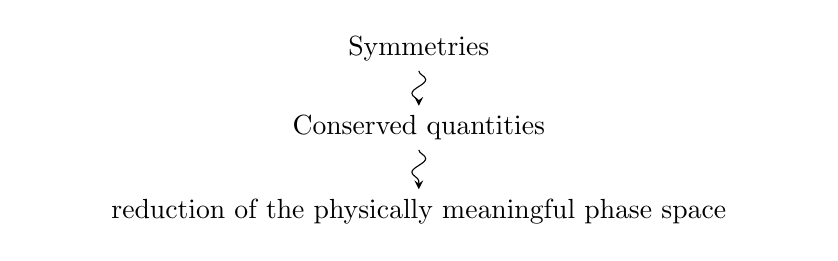
\begin{tikzpicture}[]
						\node [text width=0.8\linewidth,rectangle,align=center] (lhs) {Symmetries};
						\node [text width=0.8\linewidth, rectangle,below of=lhs,align=center] (chs) {Conserved quantities};
						\node [text width=0.8\linewidth, rectangle,below= 0.5 of chs,align=center] (rhs) {reduction of the physically meaningful phase space};
						\draw[-stealth,decorate,decoration={snake}] (lhs) -- (chs);
						\draw[-stealth,decorate,decoration={snake}] (chs) -- (rhs);
					\end{tikzpicture}						
				\end{upshotblocktitle}    	
			}
		\end{column}	
	
	\end{columns}




\end{frame}
\note[itemize]{
	\item among all possible symmetries there's a special class
	\item slogan:		Hamiltonian symmetry $\Leftrightarrow$ Admits a comoment map
	\item comomentum maps are one of the most powerful tools in the geometric mechanics toolbox
	
}
%-------------------------------------------------------------------------------------------------------------------------------------------------

%
%\begin{frame}
%						\begin{tikzpicture}
%							\pgfmathsetmacro\theta{-120}
%							\pgfmathsetmacro\viewpitch{30}
%							\pgfmathsetmacro\diam{2}
%							\pgfmathsetmacro\H{4}
%							\pgfmathsetmacro\deltaH{.5}
%							\pgfmathsetmacro\X{\diam}
%							\pgfmathsetmacro\Y{\diam*sin(\viewpitch)}	
%							\pgfmathsetmacro\vel{\diam/4}	
%													
%							
%							\draw[green,dashed,fill=green!20] (0,0) ellipse ({\X} and {\Y});
%							%\draw [blue,dashed] (-1.25,-3.5) arc (180:360:1.25 and -0.5);
%							\draw[green,dashed,fill=green!20] (0,-{\H}) ellipse ({\X} and {\Y});
%							\draw [blue,dashed] (-{\X},-{.5*\H}) arc (180:360:{\X} and -{\Y});
%		
%							\draw [green](-{\X},0) -- (-{\X},-{\H});
%							\draw [green]({\X},-{\H}) -- ({\X},0);  
%							\fill [green!80,opacity=0.5] (-{\X},0) -- (-{\X},-{\H}) arc (180:360:{\X} and {\Y}) -- ({\X},0) arc (0:180:{\X} and -{\Y});
%		
%							\draw [blue](-\X,-{.5*\H}) arc (180:360:{\X} and {\Y});
%		
%							\foreach \h in {0,-\deltaH,...,-\H}{
%								\coordinate (p) at (0,\h)++({cos(\theta)*\X},{sin(\theta)*\Y});
%								%\fill[blue] (0,\h)++({cos(\theta)*\X},{sin(\theta)*\Y}) circle(2pt);
%								\draw[red,-stealth] (0,\h)++({cos(\theta)*\X},{sin(\theta)*\Y}) --++({-\vel*sin(\theta)},{\vel*cos(\theta)*sin(\viewpitch)});
%								\draw[red] ({cos(\theta)*\X},{sin(\theta)*\Y}) -- ({cos(\theta)*\X},{sin(\theta)*\Y-\H});
%		
%						}
%		
%					    \draw[->] (5,-{\H})--(5,0) node[above] {$\dot{\Theta}$}; % ordinate
%					    \draw[->] (4,-{.5*\H})--(6,-{.5*\H})node[right] {$L$}; % ascisse
%					    \draw[-,red] (4,-{\H})--(6,0); % l'axe des abscisses
%		
%					\end{tikzpicture}		
%
%\end{frame}

%------------------------------------------------------------------------------------------------
% Frame inspired by Leonid: passing from moment maps to comoment maps
\begin{frame}[fragile]{Details: Moment maps in symplectic geometry}
	Let $(M,\omega)$ be a symplectic manifold, $\vartheta: G\times M \to M$ a Lie group action preserving $\omega$ and $v:\mathfrak{g}\to \mathfrak{X}(M)$ the corresponding infinitesimal action
	%
		\begin{defblock}[Moment map pertaining to $\vartheta$]
			Smooth map $ \mu: M \to \mathfrak{g}^\ast$ such that: \stackunder{$d \langle\mu , \xi \rangle = \iota_{v_\xi}\omega \scriptstyle\quad \forall \xi \in \mathfrak{g}$}{$f (\vartheta_g(x)) = Ad^\ast_g (f(x)) \scriptstyle\quad \forall g \in G, x \in M$}
		\end{defblock}
	%
	\vfill
	\pause
	\emph{... from a dual perspective (assuming $G$ connected) ...}
	\vspace*{-.5em}
			\begin{defblock}[Comoment map pertaining to $v$]
				\begin{columns}
					\begin{column}{.5\linewidth}	
			Lie algebra morphism \qquad $ f: \mathfrak{g} \to C^\infty(M) $
			\\
			such that \qquad $ d~f (x) = -\iota_{v_x} \omega \qquad \forall x \in \mathfrak{g}~.$
					\end{column}
					\begin{column}{.4\linewidth}	
						\begin{displaymath}
							\begin{tikzcd}
								& C^{\infty}(M,\omega) \ar[d]
								\\
								\mathfrak{g} \ar[ur,dashed,"(f)"]\ar[r,"v"']& \mathfrak{X}(M)
							\end{tikzcd}	
						\end{displaymath}
					\end{column}
				\end{columns}
		\end{defblock}		
	%
	\vfill
	\pause
	\emph{... a tool encoding conserved quantities ...}
	\vspace*{-.5em}
	\begin{propblock}[Noether Theorem]
		\small Fixed $H\in C^\infty_{\text{Ham}}(M)$ ($\mathfrak{g}$-invariant) ,
				\qquad
				$\mathcal{L}_{v_H} f(x) = 0 \qquad \forall x \in \mathfrak{g}~.$
	\end{propblock}
\end{frame}
\note[itemize]{
	\item comoment map is a Lie algebra morphism projecting to $v$. (Triangle diagram in Lie algebra category).
}
%------------------------------------------------------------------------------------------------


\end{document}